\fancyhead[L]{\textbf{\textsf{58}}}
\fancyhead[R]{\small\textsf{CHƯƠNG 1 \quad HÀM SỐ VÀ CÁC MÔ HÌNH}}
\thispagestyle{fancy}

\noindent
\begin{minipage}[t]{0.26\textwidth}
    \vspace{5.9cm}
    \centering
    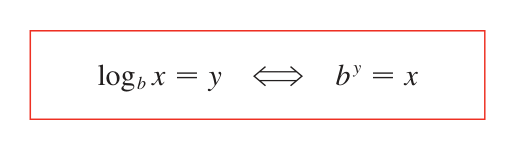
\includegraphics[width=\linewidth]{images/p0093_fig1.png}
    \vspace{1mm}
    
    \raggedright
    \textbf{\textsf{HÌNH 11}}
    
    \vspace{3.44cm}
    \textbf{\textsf{HÌNH 12}}
\end{minipage}%
\hfill
\begin{minipage}[t]{0.71\textwidth}
    khi đó ta có

    \vspace{2mm}
    \noindent
    \begin{minipage}{0.08\linewidth}
        \fcolorbox{stewartred}{white}{\bfseries\color{stewartred}6}
    \end{minipage}%
    \hfill
    \begin{minipage}{0.88\linewidth}
        \begin{tcolorbox}[colframe=stewartred,colback=white,sharp corners,boxrule=0.8pt,halign=center,top=3pt,bottom=3pt]
            $\log_b x = y \iff b^y = x$
        \end{tcolorbox}
    \end{minipage}

    \vspace{2mm}
    Do đó, nếu $x > 0$, thì $\log_b x$ là số mũ mà cơ số $b$ phải được nâng lên để thu được $x$. Chẳng hạn, $\log_{10} 0{,}001 = -3$ vì $10^{-3} = 0{,}001$.

    Các phương trình triệt tiêu (4), khi áp dụng cho các hàm số $f(x) = b^x$ và $f^{-1}(x) = \log_b x$, trở thành

    \vspace{2mm}
    \noindent
    \begin{minipage}{0.08\linewidth}
        \fcolorbox{stewartred}{white}{\bfseries\color{stewartred}7}
    \end{minipage}%
    \hfill
    \begin{minipage}{0.88\linewidth}
        \begin{tcolorbox}[colframe=stewartred,colback=white,sharp corners,boxrule=0.8pt,halign=center,top=4pt,bottom=4pt]
            \begin{tabular}{ll}
                $\log_b(b^x) = x$ & với mọi $x \in \mathbb{R}$ \\[4pt]
                $b^{\log_b x} = x$ & với mọi $x > 0$
            \end{tabular}
        \end{tcolorbox}
    \end{minipage}

    \vspace{3mm}
    Hàm logarit $\log_b$ có tập xác định là $(0, \infty)$ và tập giá trị là $\mathbb{R}$. Đồ thị của nó là ảnh phản xạ của đồ thị hàm số $y = b^x$ qua đường thẳng $y = x$.

    Hình 11 thể hiện trường hợp $b > 1$. (Các hàm logarit quan trọng nhất đều có cơ số $b > 1$.) Việc $y = b^x$ là một hàm số tăng rất nhanh khi $x > 0$ được phản ánh qua tính chất $y = \log_b x$ là một hàm số tăng rất chậm khi $x > 1$.

    Hình 12 minh họa đồ thị của hàm số $y = \log_b x$ với nhiều giá trị cơ số $b > 1$ khác nhau. Vì $\log_b 1 = 0$, nên đồ thị của mọi hàm logarit đều đi qua điểm $(1, 0)$.

    \begin{center}
        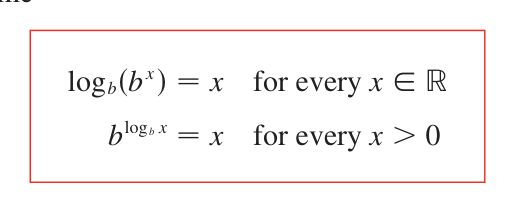
\includegraphics[width=0.72\linewidth]{images/p0093_fig2.png}
    \end{center}

    Các tính chất sau đây của hàm logarit được suy ra trực tiếp từ các tính chất tương ứng của hàm mũ đã nêu trong Mục 1.4.

    \vspace{2mm}
    \begin{tcolorbox}[colframe=stewartred,colback=white,sharp corners,boxrule=0.8pt,top=6pt,bottom=6pt,left=8pt,right=8pt]
        \noindent{\bfseries\color{stewartred}Các quy tắc logarit}\quad Nếu $x$ và $y$ là các số dương, khi đó
        \begin{enumerate}[label=\textbf{\arabic*.},itemsep=2pt,topsep=3pt,leftmargin=1.8em]
            \item $\log_b(xy) = \log_b x + \log_b y$
            \item $\log_b\left(\dfrac{x}{y}\right) = \log_b x - \log_b y$
            \item $\log_b(x^r) = r\log_b x \quad \text{(với $r$ là một số thực bất kỳ)}$
        \end{enumerate}
    \end{tcolorbox}

    \vspace{3mm}
    \noindent
    \textbf{\textsf{\color{stewartcyan}VÍ DỤ 6}} \quad Sử dụng các quy tắc logarit để tính giá trị biểu thức $\log_2 80 - \log_2 5$.

    \medskip
    \noindent
    \textbf{\textsf{\color{stewartcyan}LỜI GIẢI}} \quad Áp dụng Quy tắc 2, ta có
    \[
    \log_2 80 - \log_2 5 = \log_2\left(\frac{80}{5}\right) = \log_2 16 = 4
    \]
    vì $2^4 = 16$. \hfill {\color{stewartcyan}$\blacksquare$}
\end{minipage}